In Abbildung \ref{fig:Schaltbild} wird der Gleichstrommotor des Umwuchtsystems, vereinfacht durch das physikalische Modell einer Nebenschlussmaschine dargestellt. Diese besteht aus einem Wicklungssystem des Ankerkreises und einer Erregerwicklung, welche dem Motor parallel geschaltet ist. Aufgrund von Wicklungen und Streufeldern im Ankerkreis entsteht eine Induktivität $L_A$, über welche die Spannung $U_L$ abfällt. Dazu ist ein Widerstand $R_A$ geschaltet. Der Gleichstrommotor wird dabei ausschließlich von der Klemmspannung $U$ gesteuert. \\

\begin{figure}[!hbt]
	\centering
	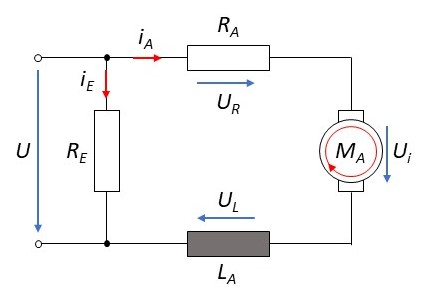
\includegraphics[width=0.5\linewidth]{Images/ProjektB_Elektrik_Ph_Modell_Schaltplan}
	\caption{Physikalisches Modell einer Nebenschlussmaschine}
	\label{fig:Schaltbild}
\end{figure}

Die gegebenen Systemparameter lauten dabei:

\begin{table}[!hbt]
	\centering
	
	\begin{tabular}{| l | l |}
		\hline
		Ankerflussverkettung, Motorkonstante & $M_A = 50 \frac{\newton\meter}{\ampere}$ \\
		\hline
		Ohmscher Widerstand des Ankerkreises & $R_A = 0.1 \ohm$ \\
		\hline
		Induktiver Widerstand des Ankerkreises & $L_A = 10 \frac{\volt\second}{\ampere} = 10 \henry$ \\
		\hline
		Klemmspannung & $U = 100 \volt$ \\
		\hline
	\end{tabular}
\captionabove{Systemparameter des physikalischen Modells für die Nebenschlussmaschine}
\label{tab:SystemparameterPH}
\end{table}
